\chapter{Implementation}\label{ch:implementation}

\subsection*{Chromosom Representation}
Wir erinnern uns, dass bei einem genetischen Algorithmus die Parameter in eine genetische Representation (Chromosom) überführt werden müssen. Die am häufigsten verwendete genetische Representation von HMM Parametern ist es die Matrizen der Parameter zu linearisieren und zu konkatenieren. Auch in dieser Arbeit werden wir solch eine Representation verwenden. Neben den parametern des Hidden Markov Models werden noch zusätzliche Informationen als Gene Kodiert. Darunter sind Fitness und Rang so wie Anzahl der Zustände und Anzahl der Emissionssymbole. Die Anzahl der Zustände und Emissionsymbole werden als Gene kodiert, damit diese bei der Überführung von Chromosom-Representation zu HMM-Representation nicht als Parameter übergeben werden müssen. Die Kodierung der Fitness und des Rangs als Gene folgt einem ähnlichen Rational.
\begin{figure}[h!]
    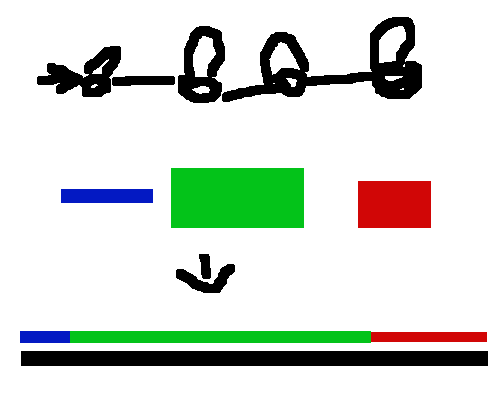
\includegraphics[scale=1.0]{images/Hmm_Chromosom_Representation.png}
    \caption{genetische Representation eines HMM}
    \label{fig:hmm_genetic_representation}
\end{figure}

\subsection*{Daten}
sooos
% \begin{lstlisting}[language=python]
%     dataset = Dataset('fsdd', n_symbols=128)
%     observations = dataset.get_first_n_observations_of_category(category_index=0, n=10)
% \end{lstlisting}

\subsection*{Architektur des GA}
Das Hauptaugenmerk der Implementation lag auf Flexibilität. Die genetischen Operatoren also Crossover, Mutation und selektion werden als callbacks einer GA-HMM instanz festgelegt. Um den Constructor einer 


\subsection*{Trainingsdaten}
Zum Evaluieren der verschiedenen Trainingsverfahren wurden zwei Datensätze erstellt. Ein Datensatz wurde aus sprachlichen Äußerungen der Zahlen 0 bis 9 erstellt. Dazu wurden die Audiodateien zunächst in eine Vektorrepresentation überführt. Sogenannte \textbf{Mel Frequency Cepestral Coefficients (MFCCs)}. Dabei handelt es sich um eine Darstellung des Frequenzspektrums welche dem menschlichen Hören nachempfunden ist. Diese MFCC-Vektoren wurden dann mit einem k-means Algorithmus quantisiert so dass man Observationssequenzen mit diskreten Symbolen erhält. Die Audiodateien wurden aus dem Free Spoken Digit Dataset (FSDD) entnommen. Ein zweiter Datensatz wurde aus Schwarz-Weiß Bildern von Gesichertern aus der ORL-Faces Datenbank generiert. Dazu wurden die Bilder zunächst linearisiert und anschließend wurden die Auflösung der Grau-Werte verringert um nicht allzuviele Emissionsymbole zu erhalten.

\subsection*{Implementation des Baum-Welch}
% Korrektheit der Implementation wurde verifiziert durch stamp
% Mehrere Auxiliary methoden zum trainieren mehrerer hmms gleichzeitig
Der Baum-Welch Algorithmus wurde ebenfalls in python implementiert. Mittels des Numba JIT Compilers wird dieser Python-Code während der Laufzeit zu hochperformanten C-Code kompiliert. Um Kompilationszeit bei einem initialen Funktionsaufruf zu umgehen wird der kompilierte C-Code gecached. Die Korrektheit der Implementation wurde verifiziert indem ein HMM mit der gleiche Observationssequenz und gleichen initialen Parametern wie in Stamp [HIER STAMP REF EINFÜGEN] trainiert wurde. Die trainierten Parameter meiner Implementation weichen von den trainierten Parametern in Stamp um weniger als 0.0001 ab, was nach 100 Iterationen wohl im Bereich der durch Systemunterschiede erklärbaren Diskrepanz liegt.

\subsection*{Testing}
Um die Korrektheit der Implementation des GA-HMM zu verifizieren wurde ein Domänenspezifisches Test-Framework entwickelt. Die domänenspezifischen Methoden ermöglichen unter anderem Assert-Statements über Validität, Equivalenz- und Ähnlichkeit der HMM und Chromosom Datentypen zu machen. Dadurch ist eine übersichtliche Validierung des Codes möglich.